%# -*- coding: utf-8-unix -*-
\chapter{单体船的窄V字形尾迹}
\label{chap:monohull}

本章考虑在无限深广的静水中匀速直线航行的单体船的窄V字形尾迹。
船体周围的流场以分布在船体表面的点源产生的流场表示,而不是简化为位于船首区域
的一个点源和位于船尾区域的一个点汇。单体船Kelvin波系中波高最大的波浪所处的射线
与航迹的夹角,即主要兴波角$\psi_{\max}$,通过一种实际的数值方法确定。
这种数值方法只涉及初等运算,因此能够被简单有效地应用。这种方法随后被用于对主尺度
范围广泛的七艘船分别在十个Froude数情况下进行系统的数值计算。
数值研究表明,船体形状的变化对主要兴波角$\psi_{\max}$的影响很弱。
一个有用的实际结果是,一般单体船的主要兴波角$\psi_{\max}$均可通过简单的解析式确定。
这些解析式为主要兴波角$\psi_{\max}(F)$提供了相对精确的实用估计(无需计算)。
这些主要兴波角$\psi_{\max}(F)$的实用解析式同时考虑了首尾散波系的纵向干涉效应和
由左右舷侧产生的波浪的横向干涉效应。因此,由此得到的主要兴波角的解析式比
两点兴波模型\supercite{Noblesse2014Why}的预测更加精确。

\section{主要兴波角的确定}
\label{sec:psimaxcalc}

由第\ref{chap:fsG}章的结果可知,只考虑速度势的波浪成分可将船后的波浪势
$\tilde{\phi}^W$写成如下Fourier-Kochin表达式
\begin{equation}
  \tilde{\phi}^W(\tilde{\mathbf{x}})=\frac{F^2}{\pi}\mathrm{Im}
  \int_{-\infty}^{\infty}
  A(q)\tilde{E}(q,\tilde{\mathbf{x}})\,\mathrm{d}q
  \label{eq:fkrepresent}
\end{equation}
其中基波$\tilde{E}(q,\tilde{\mathbf{x}})$由\eqref{eq:Etilde}给出,
波幅$A(q)$由\eqref{eq:Asymmetry}给出。这里已经忽略式\eqref{eq:phiW}中的
短波过滤函数$\tilde{\Lambda}(q,\tilde{\mathbf{x}})$,并将积分上下限由
$\pm q_{\infty}$改为$\pm\infty$。
同样处理式\eqref{eq:fsheight}可得自由面升高
\begin{equation}
  z(\tilde{x},\tilde{y})=\frac{F^2}{\pi}\mathrm{Re}\int_{-\infty}^{\infty}
  \sqrt{1+q^2}A(q)\mathrm{e}^{\mathrm{i}\sqrt{1+q^2}(\tilde{x}+q\tilde{y})/F^2}
  \,\mathrm{d}q
  \label{eq:freesurfelev}
\end{equation}

式\eqref{eq:freesurfelev}可以改写成下式
\begin{equation}
  \frac{Zg}{V^2}=\frac{1}{\pi}\mathrm{Re}\int_{-\infty}^{\infty}
  \sqrt{1+q^2}A\mathrm{e}^{\mathrm{i}h\varphi}\,\mathrm{d}q
  \label{eq:ZgV2}
\end{equation}
这里$h$是以速度无因次化的距离
\begin{eqnarray}
  && h\equiv Hg/V^2\equiv \sqrt{\xi^2+\eta^2}\label{eq:h}\\
  && (\xi,\eta)\equiv (\tilde{x},\tilde{y})/F^2\equiv(\tilde{X},\tilde{Y})g/V^2
  \label{eq:xieta}
\end{eqnarray}
$A$由式\eqref{eq:Asymmetry}定义。相位函数$\varphi$和它的一阶导数
$\varphi'\equiv\mathrm{d}\varphi/\mathrm{d}q$、二阶导数$\varphi''\equiv\mathrm{d}^2\varphi/\mathrm{d}q^2$由式\eqref{eq:faz}定义。在远场$1\ll h$,积分\eqref{eq:ZgV2}
可由第\ref{chap:shipwav}章介绍的驻相法得到解析近似
\begin{eqnarray}
  &&\frac{Zg}{V^2}\approx\sqrt{\frac{2/\pi}{h}}\mathrm{Im}(e^D+e^T)\quad\text{其中}
  \label{eq:ZgV2stat}\\
  &&e^D\equiv A^D\sqrt{\frac{1+(q^D)^2}{\varphi''_D}}\mathrm{e}^{\mathrm{i}h\varphi^D+\pi/4}\label{eq:eD}\\
  &&e^T\equiv A^T\sqrt{\frac{1+(q^T)^2}{-\varphi''_T}}\mathrm{e}^{\mathrm{i}h\varphi^T-\pi/4}\label{eq:eT}
\end{eqnarray}
这里$q^D$和$q^T$由式\eqref{eq:qTD}定义,$A^D$和$A^T$是波幅函数$A$在
$q=q^D$和$q=q^T$处的值。渐近近似\eqref{eq:ZgV2stat}在Kelvin臂附近无效,
因为在Kelvin臂二阶导数$\varphi''_D$和$\varphi''_T$为零,正如第\ref{chap:shipwav}
章所述和众所周知的。此后忽略远场驻相法近似\eqref{eq:ZgV2stat}中的横波$e^T$,
因为在高Froude数情况下,除非在Kelvin臂$\psi=\pm\psi^K$附近,散波占支配地位。
而正如前面指出的,主要兴波角$\psi_{\max}$显著小于Kelvin角$\psi^K$,
因此这种简化是合理的。在Kelvin臂附近时,横波的重要性增加,更准确的分析需要考虑横波。

图\ref{fig:psimaxmonohull}描画了由型宽$b=0.15$型深$d=0.05$的简单船体
\begin{equation}
  y=\pm\frac{b}{2}(1-16x^4)\left(1-\frac{z^2}{d^2}\right)
  \label{eq:simphull}
\end{equation}
在六个Froude数$F=$0.65,0.7,0.9,1.1,1.3和1.5时
产生的散波的波幅函数$\zeta^D\equiv\sqrt{2/\pi}F^2|e^D|$,即
\begin{equation}
  \zeta^D\equiv\sqrt{2/\pi}F^2|A^D|\sqrt{[1+(q^D)^2]/\varphi''_D}
  \label{eq:zetaD}
\end{equation}
%
\begin{figure}[htp]
  \centering
  \captionstyle{\centering}
  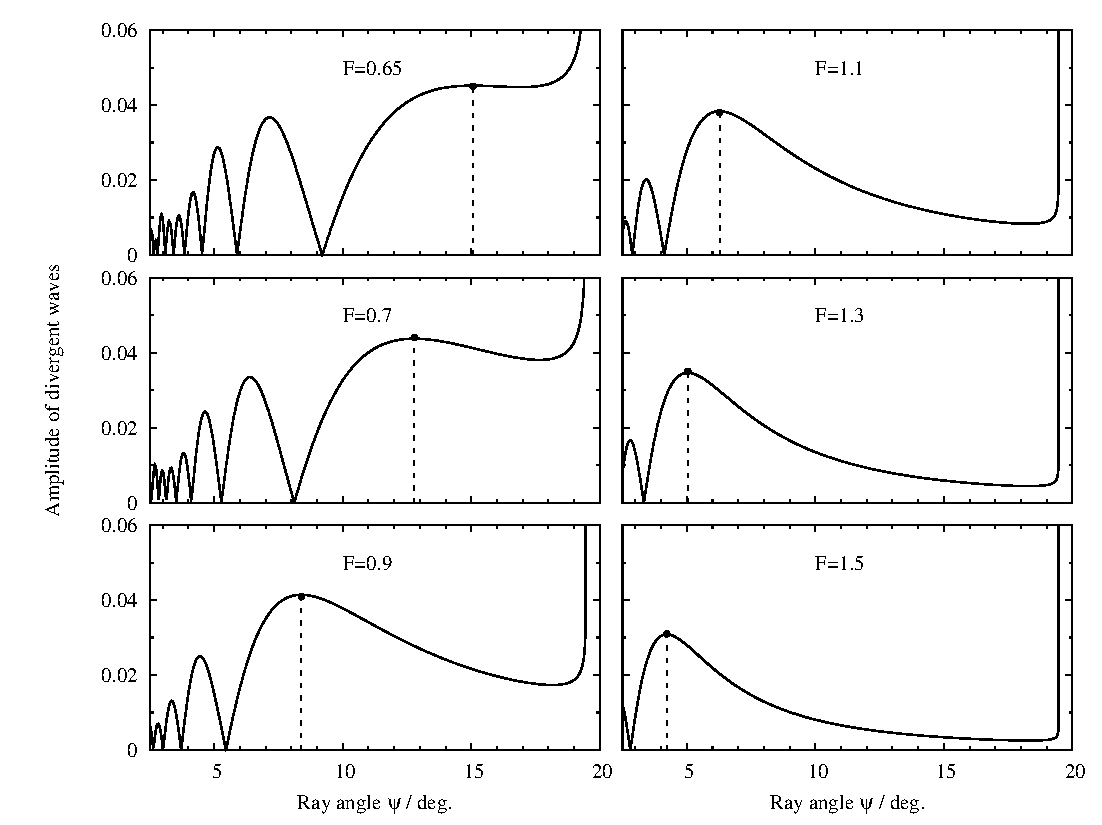
\includegraphics[width=0.8\textwidth]{chap5/amplfunc.pdf}
  \bicaption[fig:psimaxmonohull]{单体船散波的波幅函数}
  {船体\eqref{eq:simphull}在$0.65\le F\le 1.5$范围内六个Froude数情况下产生的散波的
  波幅函数$\zeta^D$,由式?定义,通过Hogner近似计算}{Fig}
  {Amplitude $\zeta^D$ of the divergent waves, defined by \eqref{eq:zetaD}, 
  created by the hull ? and predicted by the Hogner approximation, 
  for $2^\circ30'\le\psi<19^\circ28'$ and six Froude numbers $F$ within the range 
$0.65 \le F \le 1.5$}
\end{figure}

最大波高的波浪所在的射线角$\psi=\psi_{\max}$由波幅函数\eqref{eq:zetaD}
的最高峰确定。此最高峰也是最靠近Kelvin臂的`第一峰',在图\ref{fig:psimaxmonohull}
由一个点和一根竖虚线表示。正如已经指出的,二阶导数$\varphi''_D$在Kelvin臂
$\psi\approx19^\circ28'$为零,此时函数\eqref{eq:zetaD}是无界的。
图\ref{fig:psimaxmonohull}表明通过波幅函数最高峰的位置确定的主要兴波角
$\psi_{\max}$不受函数\eqref{eq:zetaD}在Kelvin臂的弱奇异性的明显影响,
除非可能对$F=0.65$。图\ref{fig:psimaxmonohull}还表明$F\ge0.9$时第一峰锐利,
并显著高于所有其他峰,但在$F\le0.7$时第一峰较宽,并且高出其他峰不多。

\section{数值计算}
\label{sec:numcomput}



